\documentclass{standalone}

\usepackage{pgf}
\usepackage{pgfpages}


\usepackage{amsmath}
\usepackage{amssymb}



\usepackage{amsthm}
\usepackage{thmtools}

%\usefonttheme{professionalfonts} % using non standard fonts for beamer
%\usepackage{fontspec}
%\setmainfont{Source Sans Pro}

% everyone:
\usepackage[utf8]{inputenc}
\usepackage[T1]{fontenc}
\usepackage{lmodern}




\usepackage{xcolor}
\usepackage{multicol}
\usepackage{wrapfig}
\definecolor{ggorange}{RGB}{237,116,108} % trouvé les couleurs dans colorimètre numérique, avec sRVB
\definecolor{ggblue}{RGB}{88,192,197} 
\newcommand{\dred}[1]{\begin{color}{red}{#1}\end{color}}
\newcommand{\dblue}[1]{\begin{color}{blue}{#1}\end{color}}
\usepackage{tikz}
\usepackage{pgfplots}
\usetikzlibrary{arrows,backgrounds,decorations}
\usepackage{tikzsymbols}

\usepackage{environ} % useful for the "scaletikzpicturetowidth" commands



\newcommand{\target}[1]{%
	\foreach \r/\col in {2.5/blue!10!white, 2/blue!20!white, 1.5/white, 1/red!10!white, 0.5/red!30!white, 0.05/red!50!white} {
		\draw [
		fill = \col%,
		% fill opacity = 0.15
		] (0, 0) circle (\r cm);
	}
}%

\newcommand{\points}[3]{%
	\foreach \i in {1, 2, ..., 20} {
		\pgfmathsetmacro{\xcoord}{#1 + rand * #3}
		\pgfmathsetmacro{\ycoord}{#2 + rand * #3}
		\draw[fill = red] (\xcoord, \ycoord) circle (2pt);
	}
}%


\newcommand{\circlevar}[3]{%
	\draw[color = green] (#1, #2) circle (#3 cm);
	\node[text = green] at (#1, #2) {$\bullet$};
}%

\def\border{
	\draw (-2.65, -2.75) -- ++(5.25, 0);
	\draw (2.75, 2.65) -- ++(0, -5.25);
}

\begin{document}

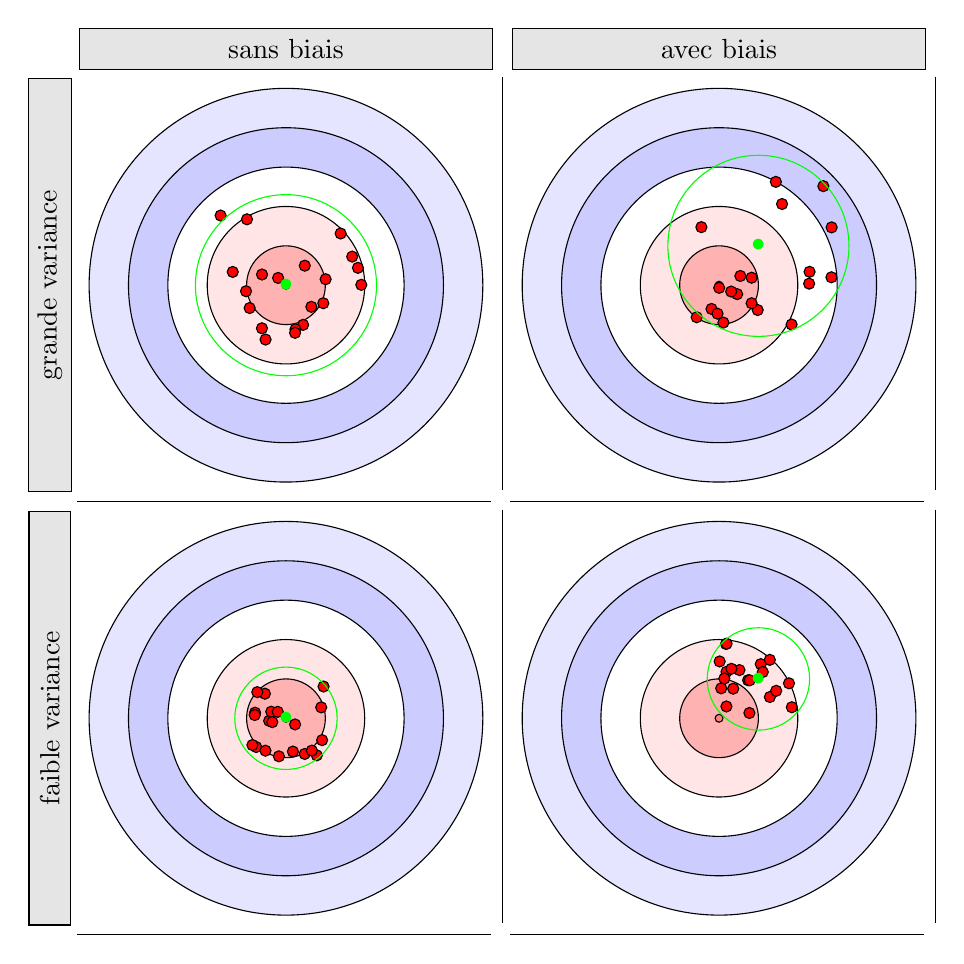
\begin{tikzpicture}[
  labeltext/.style = {
    draw, minimum width = 5.25cm, minimum height = 1.5em, fill = gray!20,
  }]
\pgfmathsetseed{1}%Setting the seed                         
\def\dist{5.5};

\begin{scope}[shift = {(0, 0)}]

  \node[labeltext] at (0, 3) {sans biais};
  \node[labeltext, rotate = 90] at (-3, 0) {grande variance};
  \target

  \points{0}{0}{1}

  \circlevar{0}{0}{1.15}
  \border
\end{scope}

\begin{scope}[shift = {(\dist, 0)}]

  \node[labeltext] at (0, 3) {avec biais};
  \target 

  \points{0.5}{0.50}{1}

  \circlevar{0.5}{0.50}{1.15}
  \border
\end{scope}

\begin{scope}[shift = {(0, -\dist)}]

  \node[labeltext, rotate = 90] at (-3, 0) {faible variance};
  \target

  \points{0}{0}{0.5}

  \circlevar{0}{0}{0.65}
  \border
\end{scope}

\begin{scope}[shift = {(\dist, -\dist)}]

  \target

  \points{0.5}{0.5}{0.5}

  \circlevar{0.5}{0.50}{0.65}
  \border
\end{scope}

\end{tikzpicture}

\end{document}